% 逻辑主线: 现有方法的不足是什么?创新设计可以如何让小设备参与大模型?

% 第5章:现有联邦学习方法的限制与突破
\subsection{Collaborative Training at Edges}\label{subsec:collaborative_training}

To harness the potential of vast amounts of data distributed across numerous devices, we envision a future where everyone can participate in training large-scale models. Federated learning emerges as a paradigm for distributed collaborative training that makes this vision possible.

% 4.3 联邦学习: 保护隐私与聚合分散数据
\textbf{Federated learning} \cite{mcmahan2017communication} is a practical paradigm that enables collaborative model training while preserving data privacy. Instead of collecting raw data from edge devices, which may violate privacy regulations like GDPR \cite{gdpr}, this approach distributes the training process across multiple devices. Each device trains on its local data and only shares model updates with the central server. This approach can effectively utilizes both computational and data resources available at edges.


\textbf{Federated LLMs for fine-tuning}
has emerged as a critical direction in recent research of large language models, addressing the challenges of privacy preservation and resource constraints. FedLLM \cite{wu2024fedllm} introduces a novel framework that enables efficient fine-tuning of large language models in a federated setting, demonstrating comparable performance to centralized fine-tuning while maintaining data privacy. FedFM \cite{chen2024fedfm} tackles the critical challenges of system and statistical heterogeneity in federated learning, proposing adaptive optimization techniques that improve model convergence across diverse client devices.
To address the computational constraints of edge devices, FedPET \cite{li2024fedpet} employs parameter-efficient fine-tuning techniques, significantly reducing the memory and computation requirements while maintaining model performance. This approach enables even resource-constrained devices to participate in the fine-tuning process. Similarly, \cite{xu2024fedfm} bridges the gap between federated learning and foundation models by introducing novel techniques for efficient knowledge transfer and model adaptation in distributed settings.
In domain-specific applications, FedQA \cite{wang2024fedqa} demonstrates the effectiveness of federated learning for question-answering tasks, showing that models can be fine-tuned on sensitive domain-specific data while preserving privacy. These advancements are supported by open-source frameworks like Flower \cite{Flower} and FATE-LLM \cite{fan2023fate}, which provide robust platforms for implementing federated fine-tuning of large language models. 



\textbf{Federated LLMs for pretraining} 
have opened up exciting new possibilities for large language model training. Rather than relying on traditional data center approaches, researchers have developed innovative geographically distributed frameworks that enable collaborative training across many devices.
% This shift represents a fundamental change in how we think about training large models, moving away from centralized computation towards more distributed, privacy-preserving architectures that can potentially leverage the computational resources of millions of edge devices.
% Recent advancements in decentralized and federated learning frameworks have made significant strides in the training of large-scale models. 
Notably, Prime Intellect \cite{OpenDiLoCo} has launched the first decentralized training project for a 10 billion parameter model, named INTELLECT-1, which utilizes the OpenDiLoCo framework to significantly reduce communication costs between nodes. This innovative approach allows for dynamic management of computational resources across multiple locations, achieving an impressive 83\% overall computational utilization while collaborating with up to 112 H100 GPUs across five countries and three continents. The model not only enhances parameter efficiency by 25 times but also demonstrates robust performance in various benchmark tests.
In parallel, the Flower Lab \cite{Flower} has introduced FlowerLLM, which successfully trained a 1.3 billion parameter large language model (LLM) using novel federated learning methods. 
Additionally, it has also developed Photon \cite{sani2024photon}, an open-source framework that provides flexible configurations for training models of different sizes, making federated LLM training more accessible to a broader range of participants and computational resources.

These frameworks underscore a shift towards decentralized AI inference and training (summarized in Appendix~\ref{app:distributed_collaborative_frameworks}), enabling researchers worldwide to contribute to advanced model development without the constraints of centralized resource control, thus paving the way for a more collaborative and inclusive AI landscape.


% Several key challenges persist in federated learning systems. Statistical heterogeneity, characterized by the non-IID (Independent and Identically Distributed) nature of data across different devices, can lead to model convergence issues and reduced performance \cite{li2020federated}. Communication efficiency remains a significant concern, as the frequent exchange of model updates between devices and the central server creates substantial communication overhead, particularly in large-scale deployments. System heterogeneity introduces additional complications, where variations in device capabilities, network conditions, and resource availability can significantly impact training efficiency and model performance. Privacy vulnerabilities also exist - while raw data remains local, sophisticated attacks (such as model inversion or membership inference) may still compromise privacy through the analysis of model updates \cite{lyu2020threats}. Finally, model complexity poses a fundamental challenge, as training large-scale models (like LLMs) through federated learning remains difficult due to the computational and memory constraints of edge devices.

% Despite these limitations, ongoing research continues to address these challenges through improved algorithms, communication protocols, and privacy-preserving techniques. The development of more efficient federated learning approaches, combined with the increasing computational capabilities of edge devices, suggests a promising future for privacy-preserving distributed AI training.

% 5.1 现有方法的不足
% \textbf{Limitations of Existing Methods}
% % - 传统联邦学习模型为什么不适合超大模型?(算力、带宽和时间差异)
% % - 客户端设备的异质性带来了哪些问题?(每个设备能否完整训练模型?)
% % - 现有方法在实际应用中可能遇到的生产环境限制是什么?

% However, traditional federated learning approaches face significant challenges when applied to large-scale models, particularly in the context of modern AI systems. The computational demands of training large models often exceed the capabilities of edge devices, creating a fundamental mismatch between model complexity and available resources \cite{kairouz2021advances}. 
% This disparity is further exacerbated by bandwidth limitations and temporal variations in network connectivity, making it impractical to synchronize model updates efficiently across distributed nodes \cite{li2020federated}.

% The heterogeneity of client devices presents another critical limitation. Edge devices vary significantly in their computational capabilities, memory capacity, and energy constraints \cite{wang2020optimizing}. This diversity makes it challenging to ensure consistent model training across all participating devices, as some may lack the resources to process even a single forward pass of the model. Furthermore, the varying processing speeds and availability patterns of devices can lead to stragglers, significantly impacting the overall training efficiency \cite{yang2019scheduling}.

% In production environments, these theoretical challenges are compounded by practical constraints. System failures, device dropouts, and network instability can disrupt the training process \cite{bonawitz2019towards}. Additionally, the need to maintain model consistency while dealing with asynchronous updates and varying data distributions poses significant challenges for deployment at scale \cite{mcmahan2017communication}.

% % 5.2 现有分布式训练框架
% \textbf{Existing Frameworks for Large Language Model Training}
% % - 总结现有大模型分布式训练框架的特点和局限性
% % - 分析它们在超大规模模型训练中的应用效果

% The training of large language models has driven the development of specialized distributed computing frameworks. These frameworks primarily focus on three key aspects: model parallelism, pipeline parallelism, and data parallelism, often combining these strategies to achieve optimal performance at scale.

% DeepSpeed \cite{rasley2020deepspeed}, developed by Microsoft, represents a comprehensive solution for training large-scale models. Its ZeRO (Zero Redundancy Optimizer) technology eliminates memory redundancy in data and model parallel training, enabling training of models with hundreds of billions of parameters. The framework's 3D parallelism combines pipeline, tensor, and data parallelism, achieving near-linear scaling efficiency. DeepSpeed has been instrumental in training models like GPT-3 and has demonstrated the ability to efficiently handle models with over a trillion parameters.

% Megatron-LM \cite{shoeybi2019megatron}, NVIDIA's contribution to large-scale model training, introduces sophisticated tensor parallelism techniques. It decomposes transformer layers across multiple GPUs, enabling efficient distributed training of massive models. The framework's integration with DeepSpeed (Megatron-DeepSpeed) has become the de facto standard for training the largest language models, combining Megatron's tensor parallelism with DeepSpeed's memory optimizations.

% Colossal-AI \cite{li2021colossal} represents a newer generation of frameworks, focusing on making large model training more accessible. It provides automatic parallelization strategies and memory management techniques, significantly reducing the engineering complexity of distributed training. The framework includes innovations like heterogeneous training support and dynamic checkpoint techniques, making it particularly suitable for academic and research environments with limited computing resources.

% Alpa \cite{zheng2022alpa} introduces a novel approach to automatic parallelization for large models. Instead of requiring manual configuration of different parallelism strategies, it automatically determines optimal parallelization plans based on the model architecture and available hardware. This automation significantly reduces the expertise required for efficient distributed training, though it may not always achieve the same performance as carefully tuned manual configurations.

% However, these frameworks still face several limitations:

% 1. Hardware Dependencies: Most frameworks are optimized for specific hardware configurations (typically NVIDIA GPUs) and may perform suboptimally on other architectures.

% 2. Complexity vs. Efficiency: While newer frameworks attempt to simplify deployment, achieving optimal performance often still requires deep expertise in distributed systems and model architecture.

% 3. Communication Bottlenecks: Despite sophisticated optimization techniques, inter-device communication remains a significant challenge, particularly in environments with limited network bandwidth.

% 4. Resource Requirements: Even with these optimizations, training large models requires substantial computational resources, limiting accessibility to organizations with significant infrastructure.

% 5.3 突破方向: 新的分布式训练范式

\section{An Open Problem: How to Train Large Language Models with Small Edge Devices?}\label{sec:open_problem}
% - 针对终端设备算力不足,量化、稀疏化、低秩矩阵技术如何应用?
% - 数据分散和异步更新环境中,训练过程如何持续迭代?(Lifelong Learning)
% - 动态扩展过程中,如何解决模型效率与性能间的平衡?

A fundamental limitation of traditional federated learning lies in its requirement for each participant to maintain and train a complete model locally. This assumption becomes particularly problematic in the context of large language models, where the computational and memory requirements far exceed the capabilities of most individual participants. For instance, in sensitive domains like healthcare~\cite{bolton2024biomedlm}, multiple hospitals may wish to collaboratively train a medical language model to leverage their collective data while maintaining data privacy. However, traditional federated learning mandates that each participating hospital possess sufficient computational resources to train the complete model locally. Despite these institutions' valuable data contributions and their motivation to enhance model capabilities through collaborative training, many hospitals lack the necessary infrastructure to participate effectively. This resource constraint significantly limits the potential for collaborative model training in critical domains where data privacy is paramount but computational resources are unevenly distributed \cite{kairouz2021advances}. 
\begin{figure}
    \centering
    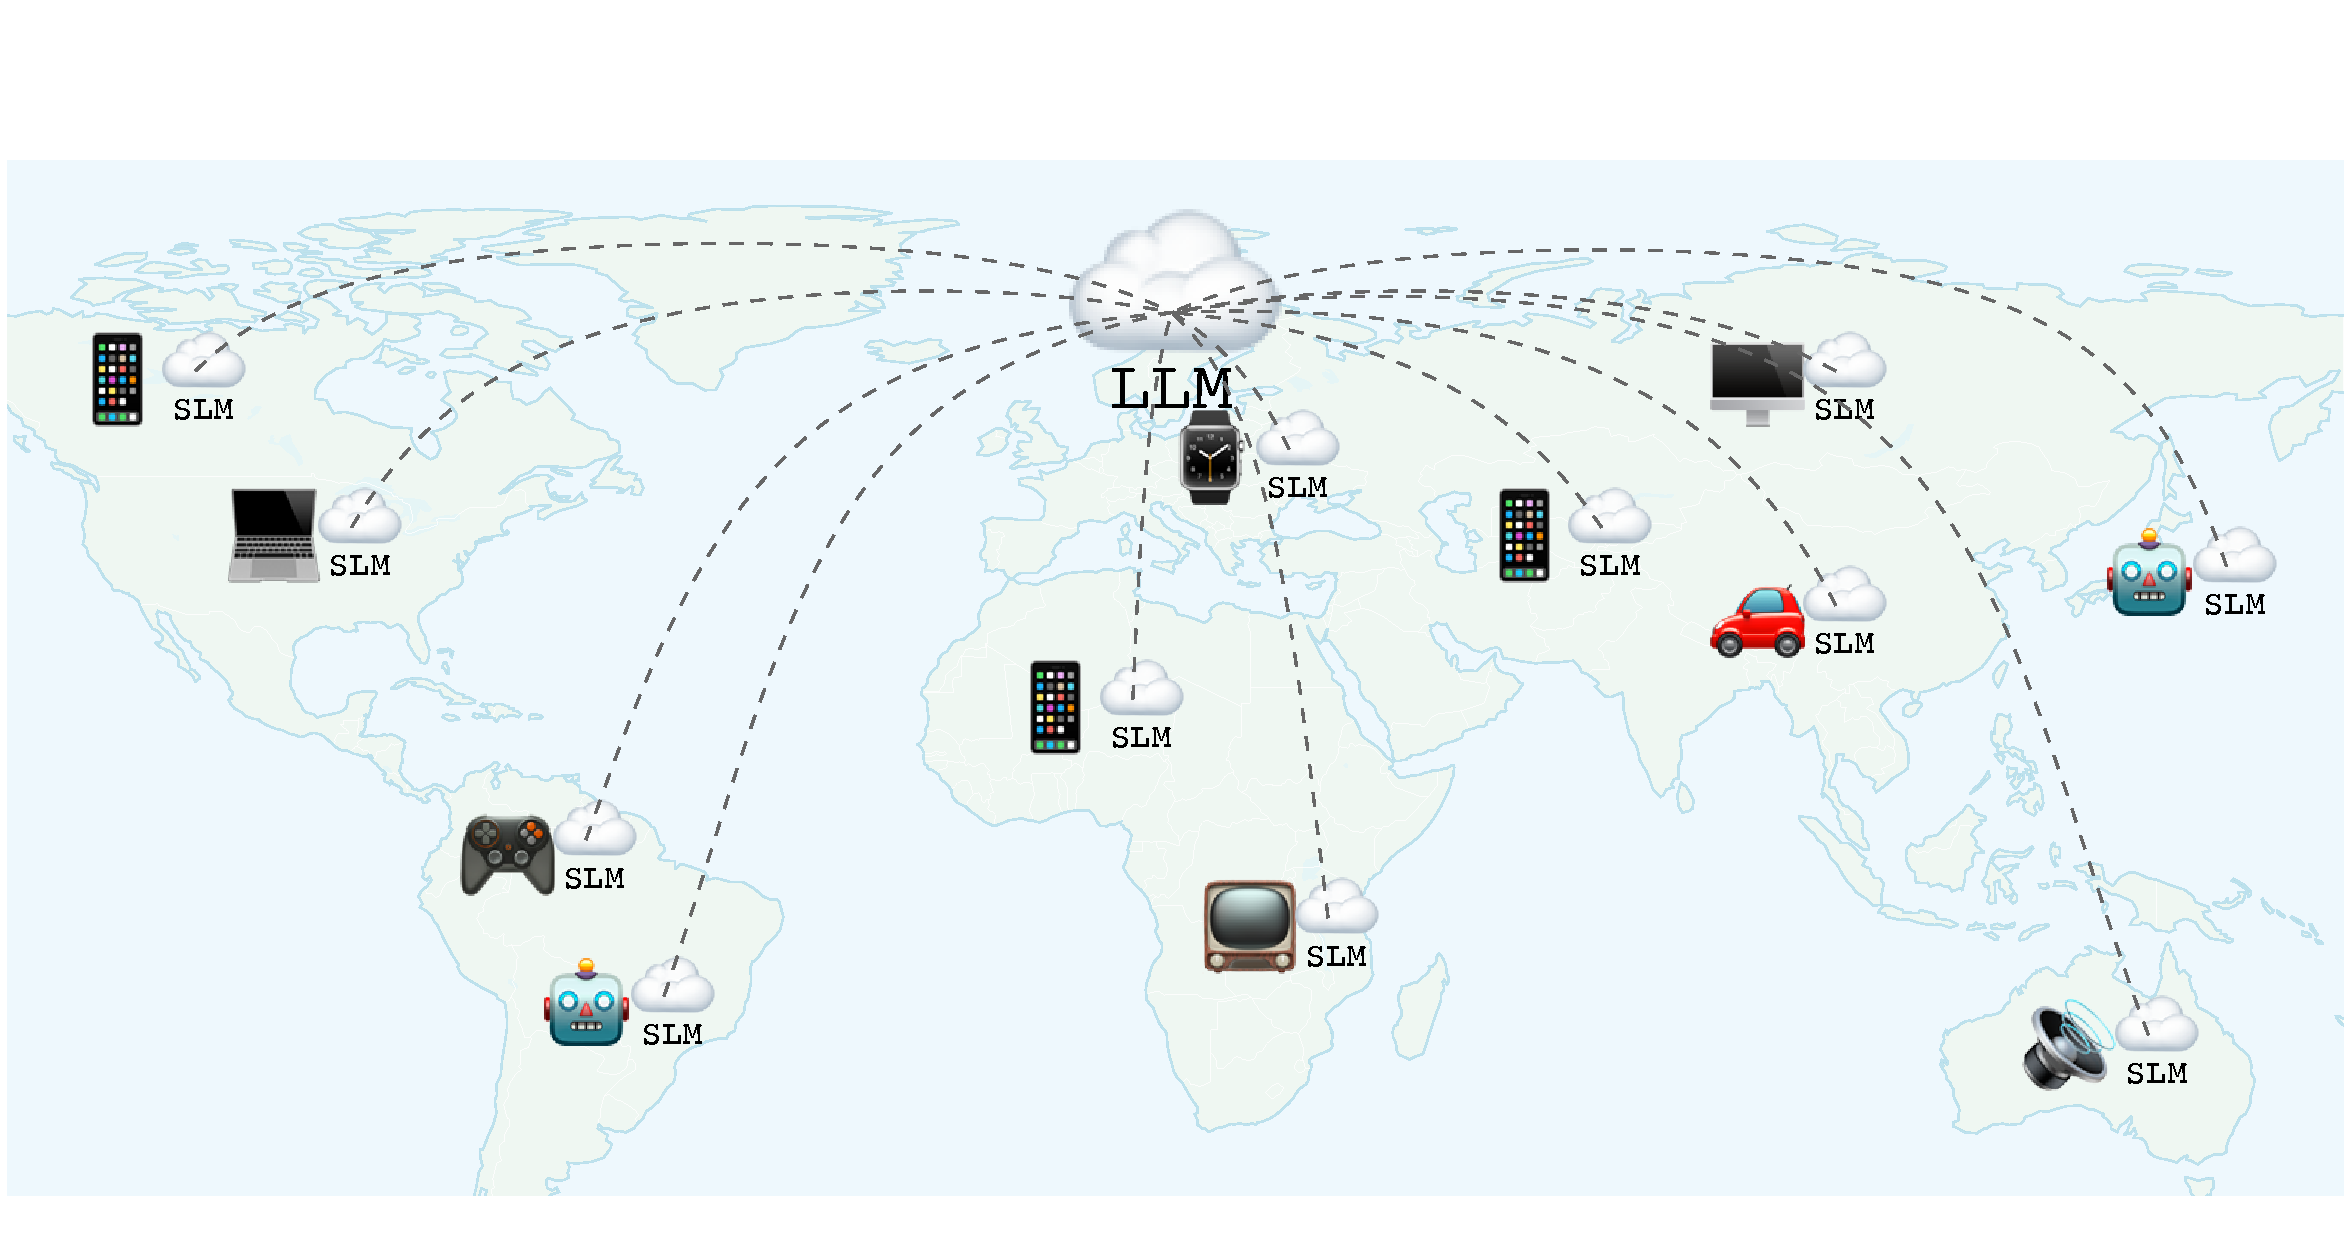
\includegraphics[width=1\linewidth]{./figs/fedllm.pdf}
    \vspace{-20pt}
    \caption{Train Large Language Models with Small Edge Devices}
    \label{fig:fedllm}
\end{figure}
While some federated learning approaches allow training partial model parameters \cite{horvath2021fjord,alam2022fedrolex}, the enormous disparity between large language models and what edge devices can train—often orders of magnitude smaller due to inherently constrained resources—remains too vast to be effectively bridged by current FL frameworks.
Therefore, we need to develop a new federated learning paradigm that enables participants to collaboratively train a large language model even under extremely limited resources (as shown in Figure~\ref{fig:fedllm}).
\textbf{It is still an open problem to train large language models with small edge devices.} Therefore, we encourage the research community to develop novel distributed collaborative computing methods in two key directions:

\subsection{Heterogeneous Device Model Fusion: \\from Small to Large}\label{subsec:model_fusion}

The first direction addresses the fundamental challenge of model size disparity in federated learning. Modern large language models typically contain hundreds of billions of parameters, while edge devices have severely limited computational resources. This creates an enormous scale gap - the large target model may be hundreds or even thousands of times larger than what individual devices can handle. To bridge this gap, each edge device should run a small language model that matches its computational capacity. For example, while the central model may have 100 billion parameters, a resource-constrained mobile device might only handle a 100-million parameter model, representing a 1000x size difference. 
The key challenge then becomes how to effectively aggregate and fuse knowledge from these much smaller models into the large target model. 
We need novel techniques that can meaningfully combine insights from models operating at radically different scales while preserving the unique contributions of each small model. This requires fundamentally rethinking traditional model fusion approaches \citep{velasevic2023effects,azizan2019distributed} to handle such extreme parameter count disparities.

\subsection{Heterogeneous Device Compute Sharing:\\ from Node to Cluster}\label{subsec:compute_sharing}

The second direction is to enable efficient compute resource sharing across heterogeneous devices by treating them as a unified compute cluster rather than independent nodes. Consider a smart home environment where multiple devices—smartphones, laptops, and desktop computers—could form a collaborative compute cluster. While each individual device has limited resources, their collective computing power could be substantial. For example, a laptop could handle intensive computational tasks, smartphones could manage coordination and lightweight processing, and desktop computers could contribute their onboard computing power. Meanwhile, other IoT devices such as smart speakers, security cameras, and vehicles could serve as data sources, providing valuable real-world inputs like voice commands, visual feeds, and environmental parameters. The language model would effectively run and train across this entire device cluster, leveraging both computing power and diverse training data from the environment.
This distributed execution requires new frameworks that can intelligently decompose and distribute model computations based on each device's capabilities and current load. The system must dynamically balance workloads - when the security cameras are idle at night, they could take on additional compute tasks, while during peak usage hours, the load could shift to other devices. 
This requires innovations in real-time resource allocation, task scheduling across heterogeneous hardware, and efficient inter-device communication protocols to ensure the collective computing power is optimally utilized \citep{zhao2024retrieval}.
% to ensure the collective computing power is optimally utilized while maintaining model coherence \citep{zhao2024retrieval}.



% To address the computational limitations of edge devices, several innovative approaches have emerged. Quantization techniques reduce model precision while maintaining performance, enabling efficient computation on resource-constrained devices \cite{zhou2016dorefa}. Similarly, model sparsification and low-rank matrix approximations offer promising directions for reducing computational and memory requirements \cite{wang2020federated}. These techniques, when combined with careful optimization, can significantly reduce the resource footprint of large models while preserving their capabilities.

% In environments characterized by distributed data and asynchronous updates, continuous learning paradigms offer a potential solution. Lifelong learning approaches enable models to adapt and improve over time, even with incomplete or inconsistent updates \cite{chen2018lifelong}. These methods incorporate mechanisms for knowledge retention and transfer, ensuring that new updates do not catastrophically interfere with previously learned information \cite{parisi2019continual}. The integration of meta-learning techniques further enhances the model's ability to adapt to new data distributions and task requirements \cite{finn2017model}.

% Balancing model efficiency and performance during dynamic scaling remains a critical challenge. Adaptive architecture techniques allow models to adjust their capacity based on available resources and task requirements \cite{tan2019efficientnet}. This flexibility enables systems to optimize resource utilization while maintaining performance standards. Furthermore, neural architecture search methods can automatically discover efficient model configurations that are well-suited to distributed training scenarios \cite{zoph2018learning}.

% 5.3 新的问题
% \textbf{Emerging Challenges}
% - 数据异质性如何解决?(各终端设备的数据分布不一致)
% - 如何处理设备异构性与异步更新问题?
% - 在一个持续学习环境中,如何动态调整模型规模?

% \textbf{Data heterogeneity} poses a fundamental challenge in federated learning systems. The non-IID nature of data across different devices can lead to divergent model updates and reduced performance \cite{zhao2018federated}. Recent research has explored techniques such as gradient normalization and personalized models to address these issues \cite{li2020federated}. However, developing robust methods that can handle extreme data heterogeneity while maintaining model performance remains an open challenge.

% \textbf{Device heterogeneity and asynchronous updates} introduce additional complexity to the training process. Variations in device capabilities and availability patterns can lead to inconsistent model updates and training instability \cite{bonawitz2019towards}. Advanced scheduling algorithms and adaptive aggregation methods have been proposed to manage these challenges \cite{yang2019scheduling}, but achieving optimal performance in highly heterogeneous environments remains difficult.

% \textbf{Continuous learning}   The ability to adjust model size and complexity in response to changing requirements and resource constraints is crucial \cite{tan2019efficientnet}. However, this flexibility must be balanced against the need for stable performance and efficient resource utilization. Research in neural architecture search and adaptive computation offers promising directions for addressing these challenges \cite{he2018amc}, but significant work remains to develop robust solutions for production environments.